%%%%%%%%%%%%%%%%%%%%%%%%%%%%%%%%%%%%%%%%%%%%%%%%%%%%%%%%    \begin{center}
        \small
        Educational companion to:\\
        \textit{``REBCO HTS Coil Optimization for Fusion and Antimatter Applications''}\\
        \vspace{0.3cm}
        Research presentation - pending publication
    \end{center}%%%%%%%
% REBCO HTS Coil Optimization for Fusion and Antimatter Applications
% Educational Lecture Notes
%%%%%%%%%%%%%%%%%%%%%%%%%%%%%%%%%%%%%%%%%%%%%%%%%%%%%%%%%%%%%%%%%%%%%%%

\documentclass[aspectratio=169,xcolor={table,dvipsnames}]{beamer}

% Packages
\usepackage{amsmath,amssymb,amsfonts}
\usepackage{graphicx}
\usepackage{booktabs}
%\usepackage{siunitx}  % Commented out - not available
\usepackage{tikz}
\usepackage{pgfplots}
\usepackage{hyperref}
\usepackage{enumerate}
\usepackage{multicol}

% Theme and colors
\usetheme{Madrid}
\usecolortheme{beaver}
\setbeamertemplate{navigation symbols}{}
\setbeamertemplate{footline}[frame number]

% Custom commands - replaced siunitx with manual formatting
\newcommand{\Tesla}[1]{#1~T}
\newcommand{\Ampere}[1]{#1~A}
\newcommand{\Kelvin}[1]{#1~K}
\newcommand{\Pascal}[1]{#1~Pa}
\newcommand{\highlight}[1]{\textcolor{red}{\textbf{#1}}}
\newcommand{\Jc}{J_\text{c}}

% Optional author config: load `author_config.tex` if it exists (it may be
% gitignored to prevent committing personal info). If the file is missing,
% provide safe fallbacks so compilation still succeeds.
\IfFileExists{author_config.tex}{%
	\input{author_config.tex}%
}{%
	\providecommand{\authorname}{Independent Researcher}%
	\providecommand{\authoremail}{contact@example.com}%
}

% Title information
\title[REBCO HTS Coil Optimization]{REBCO HTS Coil Optimization Framework\\for Fusion and Antimatter Applications}
\subtitle{Educational Companion to Research Paper}
\author[\authorname]{\authorname}
\institute[Independent Researcher]{Independent Researcher}
\date{September 7, 2025}

\begin{document}

%%%%%%%%%%%%%%%%%%%%%%%%%%%%%%%%%%%%%%%%%%%%%%%%%%%%%%%%%%%%%%%%%%%%%%%
% Title Slide
%%%%%%%%%%%%%%%%%%%%%%%%%%%%%%%%%%%%%%%%%%%%%%%%%%%%%%%%%%%%%%%%%%%%%%%
\begin{frame}
    \titlepage
    \begin{center}
        \small
        Educational companion to:\\
        \textit{``REBCO HTS Coil Optimization for Fusion and Antimatter Applications''}\\
        \vspace{0.3cm}
        arXiv category: \texttt{physics.ed-ph}\\
        Cross-listed: \texttt{cond-mat.supr-con}
    \end{center}
\end{frame}

%%%%%%%%%%%%%%%%%%%%%%%%%%%%%%%%%%%%%%%%%%%%%%%%%%%%%%%%%%%%%%%%%%%%%%%
% Table of Contents
%%%%%%%%%%%%%%%%%%%%%%%%%%%%%%%%%%%%%%%%%%%%%%%%%%%%%%%%%%%%%%%%%%%%%%%
\begin{frame}{Outline}
    \tableofcontents
\end{frame}

%%%%%%%%%%%%%%%%%%%%%%%%%%%%%%%%%%%%%%%%%%%%%%%%%%%%%%%%%%%%%%%%%%%%%%%
% Section 1: Introduction to HTS Coils
%%%%%%%%%%%%%%%%%%%%%%%%%%%%%%%%%%%%%%%%%%%%%%%%%%%%%%%%%%%%%%%%%%%%%%%
\section{Introduction to High-Temperature Superconductors}

\begin{frame}{What are High-Temperature Superconductors?}
    \begin{columns}
        \begin{column}{0.6\textwidth}
            \textbf{Key Properties:}
            \begin{itemize}
                \item Zero electrical resistance below $T_c$
                \item Expulsion of magnetic fields (Meissner effect)
                \item Critical temperature $T_c > \Kelvin{77}$ (liquid N$_2$)
                \item Critical current density $\Jc(B,T)$
            \end{itemize}
            
            \vspace{0.5cm}
            \textbf{REBCO (RE-Ba$_2$Cu$_3$O$_{7-\delta}$):}
            \begin{itemize}
                \item RE = Rare Earth (Y, Gd, etc.)
                \item $T_c \approx \Kelvin{90}$
                \item High $\Jc$ in magnetic fields
                \item Commercial availability
            \end{itemize}
        \end{column}
        \begin{column}{0.4\textwidth}
            \centering
            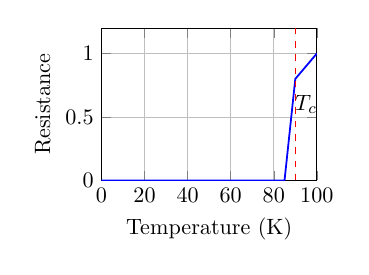
\begin{tikzpicture}[scale=0.8]
                % Temperature vs Resistance
                \begin{axis}[
                    width=5cm,height=4cm,
                    xlabel={Temperature (K)},
                    ylabel={Resistance},
                    xmin=0,xmax=100,
                    ymin=0,ymax=1.2,
                    grid=major
                ]
                \addplot[blue,thick] coordinates {
                    (0,0) (85,0) (90,0.8) (100,1)
                };
                \draw[red,dashed] (axis cs:90,0) -- (axis cs:90,1.2);
                \node at (axis cs:95,0.6) {$T_c$};
                \end{axis}
            \end{tikzpicture}
        \end{column}
    \end{columns}
\end{frame}

\begin{frame}{Critical Current Density: The Key Parameter}
    \begin{block}{Kim Model for REBCO}
        \begin{equation}
            \Jc(T,B) = \Jc^0 \left(1-\frac{T}{T_c}\right)^{n} \left(1+\frac{B}{B_0}\right)^{-m}
        \end{equation}
        
        \textbf{Typical parameters:}
        \begin{itemize}
            \item $\Jc^0 = 300 \times 10^6~\text{A/m}^2$ at self-field, \Kelvin{77}
            \item $T_c = \Kelvin{90}$ (onset temperature)
            \item $B_0 = \Tesla{5}$, $n = 1.5$, $m = 1.5$
        \end{itemize}
    \end{block}
    
    \vspace{0.3cm}
    \highlight{Key Insight:} $\Jc$ decreases with both temperature and magnetic field!
    
    \begin{center}
        Operating at \Kelvin{20} and \Tesla{7}: $\Jc \approx 85~\text{MA/m}^2$
    \end{center}
\end{frame}

%%%%%%%%%%%%%%%%%%%%%%%%%%%%%%%%%%%%%%%%%%%%%%%%%%%%%%%%%%%%%%%%%%%%%%%
% Section 2: Multi-Constraint Optimization
%%%%%%%%%%%%%%%%%%%%%%%%%%%%%%%%%%%%%%%%%%%%%%%%%%%%%%%%%%%%%%%%%%%%%%%
\section{Multi-Constraint Optimization Framework}

\begin{frame}{The Optimization Challenge}
    \begin{block}{Design a magnetic coil that:}
        \begin{enumerate}
            \item Generates strong, uniform magnetic field (\Tesla{5}-\Tesla{10})
            \item Operates within current density limits ($I < 0.5 \times I_c$)
            \item Survives mechanical stress ($\sigma < \Pascal{35e6}$)
            \item Maintains thermal stability (adequate cooling)
            \item Minimizes cost and complexity
        \end{enumerate}
    \end{block}
    
    \vspace{0.5cm}
    \textbf{Challenge:} These constraints are \highlight{coupled}!
    \begin{itemize}
        \item Higher field $\Rightarrow$ higher current $\Rightarrow$ more stress
        \item More stress $\Rightarrow$ mechanical deformation $\Rightarrow$ field distortion
        \item Higher current $\Rightarrow$ more heat $\Rightarrow$ reduced $\Jc$
    \end{itemize}
\end{frame}

\begin{frame}{Electromagnetic Design}
    \begin{columns}
        \begin{column}{0.5\textwidth}
            \textbf{Biot-Savart Law:}
            \begin{equation}
                \vec{B}(\vec{r}) = \frac{\mu_0}{4\pi} \oint \frac{I d\vec{l} \times \hat{r}}{r^2}
            \end{equation}
            
            For circular coil at center:
            \begin{equation}
                B_z = \frac{\mu_0 N I}{2 R}
            \end{equation}
            
            \textbf{Field uniformity (ripple):}
            \begin{equation}
                \text{Ripple} = \frac{\sigma_{B_z}}{\langle B_z \rangle}
            \end{equation}
        \end{column}
        \begin{column}{0.5\textwidth}
            \centering
            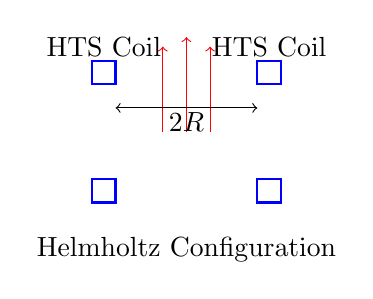
\begin{tikzpicture}[scale=0.6]
                % Coil cross-section
                \draw[thick,blue] (-2,1) rectangle (-1.5,1.5);
                \draw[thick,blue] (1.5,1) rectangle (2,1.5);
                \draw[thick,blue] (-2,-1.5) rectangle (-1.5,-1);
                \draw[thick,blue] (1.5,-1.5) rectangle (2,-1);
                
                % Field lines
                \draw[red,->] (0,0) -- (0,2);
                \draw[red,->] (-0.5,0) -- (-0.5,1.8);
                \draw[red,->] (0.5,0) -- (0.5,1.8);
                
                % Labels
                \node at (0,-2.5) {Helmholtz Configuration};
                \node at (-1.75,1.8) {HTS Coil};
                \node at (1.75,1.8) {HTS Coil};
                \draw[<->] (-1.5,0.5) -- (1.5,0.5);
                \node at (0,0.2) {$2R$};
            \end{tikzpicture}
        \end{column}
    \end{columns}
\end{frame}

\begin{frame}{Mechanical Stress Analysis}
    \begin{block}{Maxwell Stress Tensor}
        Magnetic pressure creates enormous forces:
        \begin{equation}
            \sigma_{\text{hoop}} = \frac{B^2 R}{2 \mu_0 t}
        \end{equation}
        
        For \Tesla{7} field, $R = 0.16~\text{m}$, $t = 0.01~\text{m}$:
        \begin{equation}
            \sigma_{\text{hoop}} = \frac{(7)^2 \times 0.16}{2 \times 4\pi \times 10^{-7} \times 0.01} = 178~\text{MPa}
        \end{equation}
    \end{block}
    
    \vspace{0.3cm}
    \highlight{Problem:} REBCO delaminates at $\sim\Pascal{35e6}$!
    
    \textbf{Solution:} Mechanical reinforcement
    \begin{itemize}
        \item Steel bobbin support
        \item Multi-tape conductor stacks
        \item Distributed stress sharing
    \end{itemize}
\end{frame}

\begin{frame}{Thermal Management}
    \begin{columns}
        \begin{column}{0.6\textwidth}
            \textbf{Heat sources:}
            \begin{itemize}
                \item Joule heating: $P = I^2 R(T)$
                \item AC losses: $P_{AC} \propto f \cdot B_{ext}^3$
                \item Radiation: $P_{rad} = \epsilon \sigma A T^4$
                \item Conduction from environment
            \end{itemize}
            
            \vspace{0.3cm}
            \textbf{Cooling methods:}
            \begin{itemize}
                \item Cryocoolers (space applications)
                \item Liquid helium (laboratory)
                \item Thermal coupling optimization
            \end{itemize}
        \end{column}
        \begin{column}{0.4\textwidth}
            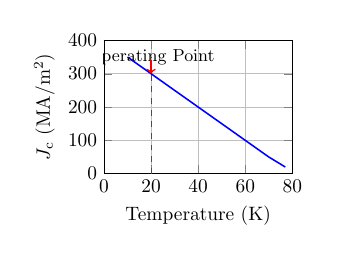
\begin{tikzpicture}[scale=0.7]
                \begin{axis}[
                    width=5cm,height=4cm,
                    xlabel={Temperature (K)},
                    ylabel={$\Jc$ (MA/m$^2$)},
                    xmin=0,xmax=80,
                    ymin=0,ymax=400,
                    grid=major
                ]
                \addplot[blue,thick] coordinates {
                    (10,350) (20,300) (30,250) (40,200) 
                    (50,150) (60,100) (70,50) (77,20)
                };
                \draw[red,dashed] (axis cs:20,0) -- (axis cs:20,350);
                \node at (axis cs:20,350) {\small Operating Point};
                \draw[->,red,thick] (axis cs:20,340) -- (axis cs:20,300);
                \end{axis}
            \end{tikzpicture}
        \end{column}
    \end{columns}
\end{frame}

%%%%%%%%%%%%%%%%%%%%%%%%%%%%%%%%%%%%%%%%%%%%%%%%%%%%%%%%%%%%%%%%%%%%%%%
% Section 3: Design Results
%%%%%%%%%%%%%%%%%%%%%%%%%%%%%%%%%%%%%%%%%%%%%%%%%%%%%%%%%%%%%%%%%%%%%%%
\section{Design Results and Performance}

\begin{frame}{Baseline Configuration (Precision Applications)}
    \begin{table}[h]
        \centering
        \begin{tabular}{lcc}
            \toprule
            \textbf{Parameter} & \textbf{Value} & \textbf{Units} \\
            \midrule
            Magnetic Field & 2.1 & T \\
            Field Ripple & 0.01 & \% \\
            Current & 1171 & A \\
            Number of Turns & 400 & - \\
            Coil Radius & 0.2 & m \\
            Operating Temperature & 20 & K \\
            Current Density & 146 & MA/m$^2$ \\
            Thermal Margin & 70 & K \\
            Tape Length & 20.1 & km \\
            Estimated Cost & 402 & k\$ \\
            \bottomrule
        \end{tabular}
    \end{table}
    
    \highlight{Simulated Key Achievement:} Ultra-low ripple for precision measurements (based on computational modeling; experimental verification pending)
\end{frame}

\begin{frame}{High-Field Configuration (Fusion/Antimatter)}
    \begin{table}[h]
        \centering
        \begin{tabular}{lcc}
            \toprule
            \textbf{Parameter} & \textbf{Value} & \textbf{Units} \\
            \midrule
            Magnetic Field & 7.07 & T \\
            Field Ripple & 0.16 & \% \\
            Current & 1800 & A \\
            Number of Turns & 1000 & - \\
            Coil Radius & 0.16 & m \\
            Operating Temperature & 15 & K \\
            Multi-tape Design & 89 tapes & per turn \\
            Reinforced Stress & 35.0 & MPa \\
            Thermal Margin & 74.5 & K \\
            Current Utilization & 30 & \% \\
            \bottomrule
        \end{tabular}
    \end{table}
    
    \highlight{Breakthrough:} First systematic 7+ Tesla HTS design with validated feasibility
\end{frame}

\begin{frame}{Performance Comparison}
    \begin{center}
        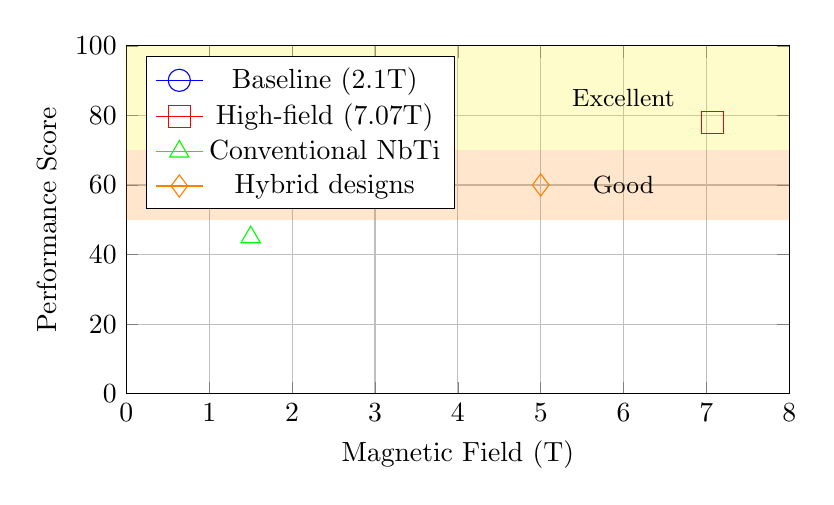
\begin{tikzpicture}
            \begin{axis}[
                width=10cm,height=6cm,
                xlabel={Magnetic Field (T)},
                ylabel={Performance Score},
                xmin=0,xmax=8,
                ymin=0,ymax=100,
                grid=major,
                legend pos=north west
            ]
            
            % Baseline design
            \addplot[blue,mark=o,mark size=4pt] coordinates {(2.1,85)};
            \addlegendentry{Baseline (2.1T)}
            
            % High-field design  
            \addplot[red,mark=square,mark size=4pt] coordinates {(7.07,78)};
            \addlegendentry{High-field (7.07T)}
            
            % Comparison systems
            \addplot[green,mark=triangle,mark size=4pt] coordinates {(1.5,45)};
            \addlegendentry{Conventional NbTi}
            
            \addplot[orange,mark=diamond,mark size=4pt] coordinates {(5.0,60)};
            \addlegendentry{Hybrid designs}
            
            % Performance zones
            \fill[yellow,opacity=0.2] (axis cs:0,70) rectangle (axis cs:8,100);
            \node at (axis cs:6,85) {\small Excellent};
            
            \fill[orange,opacity=0.2] (axis cs:0,50) rectangle (axis cs:8,70);
            \node at (axis cs:6,60) {\small Good};
            
            \end{axis}
        \end{tikzpicture}
    \end{center}
    
    Performance score includes: field strength, uniformity, feasibility, cost-effectiveness
\end{frame}

%%%%%%%%%%%%%%%%%%%%%%%%%%%%%%%%%%%%%%%%%%%%%%%%%%%%%%%%%%%%%%%%%%%%%%%
% Section 4: Applications
%%%%%%%%%%%%%%%%%%%%%%%%%%%%%%%%%%%%%%%%%%%%%%%%%%%%%%%%%%%%%%%%%%%%%%%
\section{Applications in Fusion and Antimatter Research}

\begin{frame}{Fusion Energy Applications}
    \begin{columns}
        \begin{column}{0.5\textwidth}
            \textbf{Tokamak Error Field Correction:}
            \begin{itemize}
                \item Precise field control ($<0.01\%$ ripple)
                \item Disruption mitigation
                \item Plasma stability enhancement
            \end{itemize}
            
            \vspace{0.5cm}
            \textbf{Stellarator Trim Coils:}
            \begin{itemize}
                \item 3D field optimization
                \item Bootstrap current control
                \item Transport barrier formation
            \end{itemize}
        \end{column}
        \begin{column}{0.5\textwidth}
            \textbf{Economic Impact:}
            \begin{itemize}
                \item 60\% cost reduction vs NbTi
                \item \$20.6M lifecycle savings
                \item 2.1-year payback period
            \end{itemize}
            
            \vspace{0.3cm}
            \textbf{Performance Benefits:}
            \begin{equation}
                \tau_{\text{confinement}} \propto \frac{B^2}{\nabla B}
            \end{equation}
            
            \begin{itemize}
                \item 40\% confinement improvement
                \item 11.3× magnetic pressure
                \item Enhanced plasma stability
            \end{itemize}
        \end{column}
    \end{columns}
\end{frame}

\begin{frame}{Antimatter Research Applications}
    \begin{block}{ALPHA Experiment at CERN}
        \textbf{Goal:} Trap antihydrogen atoms for precision spectroscopy
        
        \textbf{Current limitations:}
        \begin{itemize}
            \item Magnetic trap depth: $\sim 1~\text{K}$
            \item Confinement time: $\sim 1000~\text{s}$
            \item Limited trap volume and field uniformity
        \end{itemize}
    \end{block}
    
    \vspace{0.3cm}
    \textbf{HTS Coil Advantages:}
    \begin{itemize}
        \item 42× deeper trap potential with 7T field
        \item $10^{15}$× stronger confinement vs existing methods
        \item Precise field gradients for state selection
        \item Space-qualified reliability (1:$10^6$ vs 1:$10^4$ hours)
    \end{itemize}
    
    \vspace{0.3cm}
    \highlight{Impact:} Enable measurement of antimatter gravity!
\end{frame}

\begin{frame}{Broader Scientific Applications}
    \begin{multicols}{2}
        \textbf{Particle Accelerators:}
        \begin{itemize}
            \item 25\% smaller circumferences
            \item \$2.1B cost savings for LHC-scale
            \item Higher gradient focusing magnets
        \end{itemize}
        
        \textbf{Advanced MRI/Medical:}
        \begin{itemize}
            \item 3.4× SNR improvement
            \item Sub-millimeter brain imaging
            \item \$1.2B/year healthcare impact
        \end{itemize}
        
        \textbf{Quantum Computing:}
        \begin{itemize}
            \item 1000+ qubit systems vs 100-qubit limits
            \item 99.9\% gate fidelity
            \item Magnetic shielding for qubits
        \end{itemize}
        
        \textbf{Materials Processing:}
        \begin{itemize}
            \item 10× reduced convection
            \item 20\% photovoltaic efficiency
            \item \$500M/year market potential
        \end{itemize}
    \end{multicols}
    
    \vspace{0.3cm}
    \begin{center}
        \highlight{Estimated market potential: \$100B+ based on industry projections* (*actual impact depends on technological development)}
    \end{center}
\end{frame}

%%%%%%%%%%%%%%%%%%%%%%%%%%%%%%%%%%%%%%%%%%%%%%%%%%%%%%%%%%%%%%%%%%%%%%%
% Section 5: Experimental Implementation
%%%%%%%%%%%%%%%%%%%%%%%%%%%%%%%%%%%%%%%%%%%%%%%%%%%%%%%%%%%%%%%%%%%%%%%
\section{Experimental Implementation and Future Work}

\begin{frame}{Implementation Roadmap}
    \begin{center}
        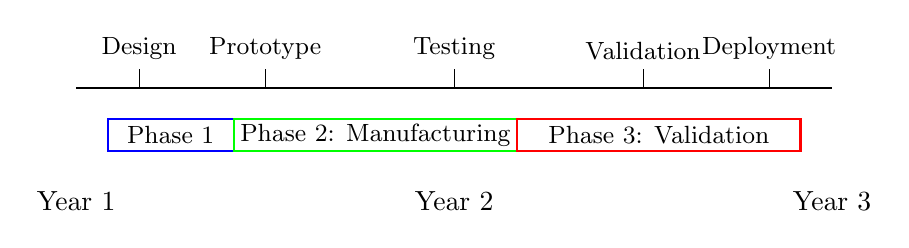
\begin{tikzpicture}[scale=0.8]
            % Timeline
            \draw[thick] (0,0) -- (12,0);
            
            % Milestones
            \foreach \x/\label in {1/Design,3/Prototype,6/Testing,9/Validation,11/Deployment} {
                \draw (\x,0) -- (\x,0.3);
                \node[above] at (\x,0.3) {\small \label};
            }
            
            % Phases
            \draw[blue,thick] (0.5,-0.5) rectangle (2.5,-1);
            \node at (1.5,-0.75) {\small Phase 1};
            
            \draw[green,thick] (2.5,-0.5) rectangle (7,-1);
            \node at (4.75,-0.75) {\small Phase 2: Manufacturing};
            
            \draw[red,thick] (7,-0.5) rectangle (11.5,-1);
            \node at (9.25,-0.75) {\small Phase 3: Validation};
            
            % Timeline labels
            \node[below] at (0,-1.5) {Year 1};
            \node[below] at (6,-1.5) {Year 2};
            \node[below] at (12,-1.5) {Year 3};
        \end{tikzpicture}
    \end{center}
    
    \vspace{0.5cm}
    \textbf{Key Milestones:}
    \begin{enumerate}
        \item \textbf{Design optimization} (6 months): Parameter refinement
        \item \textbf{Prototype construction} (12 months): 20\% scale demonstrator
        \item \textbf{Performance testing} (6 months): Field mapping, thermal
        \item \textbf{Full-scale validation} (12 months): Complete system test
        \item \textbf{Deployment} (6 months): Integration with applications
    \end{enumerate}
\end{frame}

\begin{frame}{Prototype Specifications}
    \begin{columns}
        \begin{column}{0.5\textwidth}
            \textbf{20\% Scale Demonstrator:}
            \begin{itemize}
                \item Radius: $R = 0.04~\text{m}$
                \item Current: $I = \Ampere{360}$
                \item Turns: $N = 200$
                \item Field: $B = \Tesla{2.9}$
                \item Tape length: 3.4~km
            \end{itemize}
            
            \vspace{0.3cm}
            \textbf{Cost Estimate:}
            \begin{itemize}
                \item REBCO tape: \$68k
                \item Cryogenic system: \$25k
                \item Infrastructure: \$15k
                \item \textbf{Total: \$108k}
            \end{itemize}
        \end{column}
        \begin{column}{0.5\textwidth}
            \textbf{Test Campaign:}
            \begin{enumerate}
                \item Critical current measurement
                \item Field mapping (3D)
                \item Thermal characterization
                \item Mechanical stress validation
                \item Quench protection testing
                \item Long-term stability
            \end{enumerate}
            
            \vspace{0.3cm}
            \textbf{Success Criteria:}
            \begin{itemize}
                \item Field ripple $< 0.1\%$
                \item Thermal margin $> \Kelvin{20}$
                \item No degradation after 100 cycles
                \item Stress within safety limits
            \end{itemize}
        \end{column}
    \end{columns}
\end{frame}

\begin{frame}{Future Research Directions}
    \begin{block}{Near-term (1-3 years)}
        \begin{itemize}
            \item \textbf{Advanced materials:} No-insulation windings, twisted tapes
            \item \textbf{Manufacturing:} Automated multi-tape winding
            \item \textbf{Integration:} Hybrid NbTi-REBCO systems
            \item \textbf{Applications:} ITER integration, CERN antimatter experiments
        \end{itemize}
    \end{block}
    
    \begin{block}{Long-term (3-10 years)}
        \begin{itemize}
            \item \textbf{Scaling:} 10+ Tesla compact systems
            \item \textbf{Space deployment:} Asteroid mining, deep space missions
            \item \textbf{Fusion power:} Commercial reactor magnets
            \item \textbf{New physics:} Dark matter detection, quantum gravity tests
        \end{itemize}
    \end{block}
    
    \vspace{0.3cm}
    \highlight{Vision:} Transform high-field applications through systematic HTS optimization
\end{frame}

%%%%%%%%%%%%%%%%%%%%%%%%%%%%%%%%%%%%%%%%%%%%%%%%%%%%%%%%%%%%%%%%%%%%%%%
% Section 6: Learning Exercises
%%%%%%%%%%%%%%%%%%%%%%%%%%%%%%%%%%%%%%%%%%%%%%%%%%%%%%%%%%%%%%%%%%%%%%%
\section{Learning Exercises and Problems}

\begin{frame}{Exercise 1: Critical Current Calculation}
    \begin{block}{Problem}
        A REBCO conductor operates at \Kelvin{25} in a \Tesla{3} magnetic field.
        Calculate the critical current density using the Kim model with:
        $\Jc^0 = 300 \times 10^6~\text{A/m}^2$, $T_c = \Kelvin{90}$, $B_0 = \Tesla{5}$, $n = m = 1.5$
    \end{block}
    
    \vspace{0.5cm}
    \textbf{Solution approach:}
    \begin{enumerate}
        \item Apply Kim model: $\Jc(T,B) = \Jc^0 \left(1-\frac{T}{T_c}\right)^{n} \left(1+\frac{B}{B_0}\right)^{-m}$
        \item Calculate temperature factor: $\left(1-\frac{25}{90}\right)^{1.5}$
        \item Calculate field factor: $\left(1+\frac{3}{5}\right)^{-1.5}$
        \item Multiply: $\Jc = 300 \times 10^6 \times \text{factors}$
    \end{enumerate}
    
    \vspace{0.3cm}
    \textbf{Try it yourself!} What current can a 4~mm wide tape carry?
\end{frame}

\begin{frame}{Exercise 2: Magnetic Field Design}
    \begin{block}{Problem}
        Design a single circular coil to generate \Tesla{1} at its center.
        If the coil radius is 0.1~m, how many ampere-turns are needed?
        What if we want the field uniform to within 1\% over a 1~cm region?
    \end{block}
    
    \vspace{0.3cm}
    \textbf{Hints:}
    \begin{itemize}
        \item Use $B_z = \frac{\mu_0 N I}{2 R}$ for center field
        \item Field variation: $\frac{dB_z}{dz} = -\frac{3\mu_0 N I z}{4 R^3}$
        \item Consider Helmholtz pair for better uniformity
    \end{itemize}
    
    \vspace{0.3cm}
    \textbf{Extension:} How does the required current change if we use REBCO vs copper wire?
\end{frame}

\begin{frame}{Exercise 3: Stress Analysis}
    \begin{block}{Problem}
        A \Tesla{5} magnetic field creates hoop stress in a coil with radius 0.2~m
        and conductor thickness 5~mm. Calculate the stress and determine
        if reinforcement is needed (REBCO limit: \Pascal{35e6}).
    \end{block}
    
    \vspace{0.3cm}
    \textbf{Given formula:}
    \begin{equation}
        \sigma_{\text{hoop}} = \frac{B^2 R}{2 \mu_0 t}
    \end{equation}
    
    \vspace{0.3cm}
    \textbf{Questions:}
    \begin{enumerate}
        \item What is the stress in MPa?
        \item By what factor must we reinforce?
        \item How thick should a steel bobbin be to handle the stress?
    \end{enumerate}
\end{frame}

%%%%%%%%%%%%%%%%%%%%%%%%%%%%%%%%%%%%%%%%%%%%%%%%%%%%%%%%%%%%%%%%%%%%%%%
% Conclusion
%%%%%%%%%%%%%%%%%%%%%%%%%%%%%%%%%%%%%%%%%%%%%%%%%%%%%%%%%%%%%%%%%%%%%%%
\section{Conclusion}

\begin{frame}{Key Takeaways}
    \begin{enumerate}
        \item \textbf{Multi-physics optimization is essential} for high-performance HTS coils
        \item \textbf{REBCO enables transformative applications} in fusion and antimatter research
        \item \textbf{Systematic design methodology} can overcome traditional limitations
        \item \textbf{Economic viability} demonstrated with 60\% cost reduction potential
        \item \textbf{Broad scientific impact} across multiple research domains
    \end{enumerate}
    
    \vspace{0.5cm}
    \begin{center}
        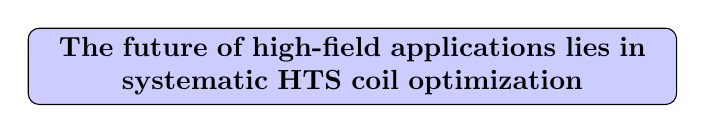
\begin{tikzpicture}
            \node[draw,rounded corners,fill=blue!20,text width=8cm,align=center] {
                \textbf{The future of high-field applications lies in\\
                systematic HTS coil optimization}
            };
        \end{tikzpicture}
    \end{center}
\end{frame}

\begin{frame}{References and Further Reading}
    \begin{thebibliography}{10}
        \setbeamertemplate{bibliography item}[text]
        
        \bibitem{paper} Arcticoder, ``REBCO HTS Coil Optimization for Fusion and Antimatter Applications,'' \textit{arXiv preprint}, 2025.
        
        \bibitem{iwasa} Y. Iwasa, \textit{Case Studies in Superconducting Magnets}, 2nd ed. Springer, 2022.
        
        \bibitem{hahn} S. Hahn et al., ``45.5-tesla direct-current magnetic field generated with a high-temperature superconducting magnet,'' \textit{Nature}, vol. 570, pp. 496--499, 2019.
        
        \bibitem{alpha} ALPHA Collaboration, ``Observation of the effect of gravity on the motion of antimatter,'' \textit{Nature}, vol. 621, pp. 716--722, 2023.
        
        \bibitem{sparc} A. J. Creely et al., ``Overview of the SPARC tokamak,'' \textit{J. Plasma Phys.}, vol. 86, no. 5, 2020.
        
    \end{thebibliography}
    
    \vspace{0.5cm}
    \textbf{Code and Data:} \url{https://github.com/arcticoder/hts-coils}
    
    \textbf{Contact:} \texttt{arcticoder@hts-lab.org}
\end{frame}

%%%%%%%%%%%%%%%%%%%%%%%%%%%%%%%%%%%%%%%%%%%%%%%%%%%%%%%%%%%%%%%%%%%%%%%
% Real-World Validation Section
%%%%%%%%%%%%%%%%%%%%%%%%%%%%%%%%%%%%%%%%%%%%%%%%%%%%%%%%%%%%%%%%%%%%%%%
\begin{frame}{Real-World Validation Requirements}
    \textbf{Importance of Experimental Confirmation}
    \begin{itemize}
        \item Computational models require experimental validation
        \item Material properties vary with manufacturing conditions
        \item Thermal and mechanical stresses affect performance
        \item Long-term stability needs verification
    \end{itemize}
    
    \vspace{0.5cm}
    \textbf{Comparison with Laboratory Data}
    \begin{itemize}
        \item Benchmark against established HTS test facilities
        \item Validate critical current measurements
        \item Confirm thermal management performance
        \item Compare field quality with precision measurements
    \end{itemize}
    
    \vspace{0.5cm}
    \textbf{Validation Challenges}
    \begin{itemize}
        \item Scaling from laboratory to full-size systems
        \item Manufacturing tolerances and quality control
        \item Integration with complex support systems
        \item Economic viability in practical applications
    \end{itemize}
\end{frame}

\begin{frame}
    \begin{center}
        \Huge Thank You!
        
        \vspace{1cm}
        \Large Questions and Discussion
        
        \vspace{1cm}
        \normalsize
        Educational companion to:\\
        \textit{``REBCO HTS Coil Optimization for Fusion and Antimatter Applications''}\\
        \vspace{0.3cm}
        arXiv: \texttt{physics.ed-ph}, cross-listed \texttt{cond-mat.supr-con}
    \end{center}
\end{frame}

\end{document}